\documentclass[11pt]{article}
\usepackage[utf8]{inputenc}
\usepackage[T1]{fontenc}
\usepackage{lmodern}
\usepackage[english]{babel}
\usepackage{amsmath,amssymb,amsthm,booktabs,graphicx,geometry}
\usepackage[round,authoryear]{natbib}
\usepackage{setspace}
\usepackage[colorlinks=true,linkcolor=black,citecolor=black,urlcolor=black]{hyperref}
\geometry{letterpaper,margin=1in}
\renewcommand{\thesection}{OA.\arabic{section}}
\renewcommand{\thetable}{OA.\arabic{table}}
\renewcommand{\thefigure}{OA.\arabic{figure}}
\newtheorem{proposition}{Proposition}
\theoremstyle{definition}
\newtheorem{definition}{Definition}
\newcommand{\JJ}{\mathcal{J}}
\newcommand{\DD}{\mathcal{D}}
% Generated by scripts/jfec_build.py -- do not edit by hand.
\newcommand{\gnSpRawNull}{-0.06}
\newcommand{\gnSpFeObs}{0.38}
\newcommand{\gnSpFeNull}{-0.02}
\newcommand{\gnSpFeShrink}{61\%}
\newcommand{\gnSpFeDevolP}{0.045}
\newcommand{\gnFfRawNull}{0.83}
\newcommand{\gnFfFeObs}{1.43}
\newcommand{\gnFfFeNull}{0.54}
\newcommand{\gnFfFeShrink}{61\%}
\newcommand{\gnFfFeDevolP}{0.129}
\newcommand{\mcSizeIidIid}{3\%}
\newcommand{\mcSizeIidFhs}{4\%}
\newcommand{\mcGarchIid}{17\%}
\newcommand{\mcGarchFhs}{6\%}
\newcommand{\mcMsvolIid}{4\%}
\newcommand{\mcMsvolFhs}{11\%}
\newcommand{\mcPowIid}{48\%}
\newcommand{\mcPowFhs}{68\%}
\newcommand{\mcWorstOne}{5\%}
\newcommand{\mcBothSizeIid}{2\%}
\newcommand{\mcBothGarch}{6\%}
\newcommand{\mcBothMsvol}{4\%}
\newcommand{\mcBothPow}{46\%}
\newcommand{\mcBothWorst}{6.5\%}
\newcommand{\mcBothWorstOne}{1.0\%}
\newcommand{\biasTwentyApprox}{0.39}
\newcommand{\biasTwentyRaw}{0.39}
\newcommand{\biasTwentyT}{0.39}
\newcommand{\biasTwentyLW}{0.002}
\newcommand{\biasFortyEightApprox}{2.41}
\newcommand{\gjrSpPers}{0.989}
\newcommand{\gjrSpAlpha}{0.033}
\newcommand{\gjrSpGamma}{0.063}
\newcommand{\gjrSpBeta}{0.920}
\newcommand{\gjrFfPers}{0.987}
\newcommand{\gjrFfAlpha}{0.030}
\newcommand{\gjrFfGamma}{0.079}
\newcommand{\gjrFfBeta}{0.916}
\newcommand{\cwSpFive}{0.000}
\newcommand{\cwSpTen}{0.001}
\newcommand{\cwFfFive}{0.000}
\newcommand{\cwFfTen}{0.000}
\newcommand{\holmNtests}{23}
\newcommand{\holmNsurv}{9}

\newcommand{\KL}[2]{D_{\mathrm{KL}}\!\left(#1\,\Vert\,#2\right)}
\begin{document}
\begin{center}
{\large\bfseries Online Appendix to\\ ``What Survives a Placebo? Entropy, Market Coupling\\ and the Plausibility of Stress Scenarios''\par}
\vspace{6pt} Sébastien Gallet \quad November 2026
\end{center}
\onehalfspacing
\noindent This appendix collects material that supports the main text but is
not needed to follow it: the dynamic postulates and the volume-time argument
behind the framework (section~\ref{oa:theory}); the full placebo tables
(section~\ref{oa:placebo}); the severity ladder, the composition of scenarios
and reverse stress testing (section~\ref{oa:ladder}); the computation of the
EBA scenario's cost (section~\ref{oa:eba}); and a euro-area application of the
block decomposition, the entropic CISS (section~\ref{oa:ciss}). Numbers are
those of the replication package. Table and figure numbers refer to this
appendix unless they are prefixed ``main text''.

\section{Dynamic postulates and the volume-time argument}
\label{oa:theory}
\subsection{The bridge from order flow to Gaussian prices}
\label{oa:pont}

Over an interval, let $V$ be traded volume and $Q$ net signed order flow (buys
minus sells). Two assumptions suffice. \emph{Linear impact}: the change in log
price is $\lambda Q$, as in \citet{kyle1985}. \emph{Variance proportional to
volume}: given $V$, the market knows only the mean of $Q$ and a variance
$\varsigma^2V$. Maximum entropy then gives
\begin{equation}
\Delta X \mid V \;\sim\; \mathcal N\!\left(\lambda m,\ \lambda^2\varsigma^2 V\right).
\end{equation}
The conditioning variable is volume, not time: this is the
mixture-of-distributions hypothesis of \citet{clark1973} and
\citet{tauchen1983}, and \citet{ane2000} show that returns measured in
transaction time are close to Gaussian. Unconditionally, the return is a
mixture of Gaussians, hence fat-tailed \citep{mandelbrot1967}: fat tails alone
do not prove that information is present. If increments are moreover
independent in volume time, the log price is a time-changed Brownian motion,
and the price a geometric Brownian motion. Both assumptions are imperfect
(real impact is closer to a square root, and order flow is autocorrelated),
which is why all empirical work is done in calendar time.

\subsection{Index dynamics: a theorem and two postulates}
\label{app:dynamique}

\paragraph{The theorem.} For a return $X$ and a signal $Y$,
$\mathbb{E}_Y[h(X\mid Y)]=h(X)-I(X;Y)\le h(X)$ \citep{cover2006}. Receiving
information lowers entropy \emph{on average} by exactly the mutual
information. A particular realisation can raise it (a confusing signal); the
jump component is therefore mainly, not exclusively, one-sided.

\paragraph{Postulate 1 (relaxation).} Without new information, $\JJ$ reverts
to a long-run level: $d\JJ_t=-\kappa(\JJ_t-\bar\JJ)\,dt+\sigma_\JJ\,dW_t$. An
Ornstein--Uhlenbeck process is the only process that is Markovian, Gaussian
and stationary \citep{doob1942}. Adding the jumps caused by news gives
\begin{equation}
d\JJ_t \;=\; -\kappa(\JJ_t-\bar\JJ)\,dt \;+\; \sigma_\JJ\,dW_t \;+\; dZ_t ,
\end{equation}
where $Z_t$ is the sum of positive jumps up to $t$: the class of
\citet{bns2001}. The half-life of a shock is $\ln2/\kappa$.

\paragraph{Postulate 2 (sign).} $\JJ$ is an even function of skewness: a
distribution with a long left tail (a crash) and its mirror image (a rally)
have the same $\JJ$. Saying anything about direction requires an outside
ingredient. We postulate that jumps come with negative skewness, relying on
the leverage effect \citep{black1976,engle1993}.

\paragraph{Why dependence and tails should rise together.} Major news hits
every asset on the same day. On that day, assets move together (coupling
rises) and each records an unusual loss (its tails fatten). The two channels
describe the same day seen from two places. In calm markets, large moves are
asset-specific and couple nothing. This is H6. The null shows, however, that
this coincidence is also produced mechanically by estimation.

\subsection{Index dynamics: a theorem and two postulates}
\label{oa:dyn}

\paragraph{The theorem.} For a return $X$ and a signal $Y$,
$\mathbb{E}_Y[h(X\mid Y)]=h(X)-I(X;Y)\le h(X)$ \citep{cover2006}. Receiving
information lowers entropy \emph{on average} by exactly the mutual
information. A particular realisation can raise it (a confusing signal); the
jump component is therefore mainly, not exclusively, one-sided.

\paragraph{Postulate 1 (relaxation).} Without new information, $\JJ$ reverts
to a long-run level: $d\JJ_t=-\kappa(\JJ_t-\bar\JJ)\,dt+\sigma_\JJ\,dW_t$. An
Ornstein--Uhlenbeck process is the only process that is Markovian, Gaussian
and stationary \citep{doob1942}. Adding the jumps caused by news gives
\begin{equation}
d\JJ_t \;=\; -\kappa(\JJ_t-\bar\JJ)\,dt \;+\; \sigma_\JJ\,dW_t \;+\; dZ_t ,
\end{equation}
where $Z_t$ is the sum of positive jumps up to $t$: the class of
\citet{bns2001}. The half-life of a shock is $\ln2/\kappa$.

\paragraph{Postulate 2 (sign).} $\JJ$ is an even function of skewness: a
distribution with a long left tail (a crash) and its mirror image (a rally)
have the same $\JJ$. Saying anything about direction requires an outside
ingredient. We postulate that jumps come with negative skewness, relying on
the leverage effect \citep{black1976,engle1993}.

\paragraph{Why dependence and tails should rise together.} Major news hits
every asset on the same day. On that day, assets move together (coupling
rises) and each records an unusual loss (its tails fatten). The two channels
describe the same day seen from two places. In calm markets, large moves are
asset-specific and couple nothing. This is H6. The null shows, however, that
this coincidence is also produced mechanically by estimation.


\section{Full placebo tables and estimation details}
\label{oa:placebo}
\subsection{Empirical details}


\paragraph{Estimators.} Two covariance estimators run in parallel: a 252-day
rolling window with the \citet{ledoit2004} correction, and exponential
weighting with a 60-day half-life and $10\,\%$ shrinkage towards the diagonal.
The second prevents an extreme day \emph{leaving} the window from creating a
false jump. The shape deficit uses the \citet{hyvarinen1998} approximation,
whose two terms separate a skewness channel and a tail channel; the better
known Edgeworth expansion $S^2/12+K^2/48$ overstates the deficit of a
Student~$t$ with 4 degrees of freedom by a factor of 69. Jumps are detected at
four times a local scale given by bipower variation lagged by one day
\citep{bns2004}.

\paragraph{Inference.} Two consecutive rolling windows share 251 of their
252~days. Regime comparisons therefore use a circular block bootstrap with
252-day blocks. The relaxation $p$-value follows the Dickey--Fuller
distribution. Forecasts (H7) are re-estimated every year on the past and
compared on dates spaced by the forecast horizon, with the \citet{dm1995}
test.

\paragraph{Raw stress-regime results (S\&P~500).} Under stress ($1,076$ dates
against $6,481$), scale rises by $5.97$~nats, dependence falls by $0.99$,
shape rises by $0.27$ ($p=0.16$), and $\JJ$ rises by $1.94$ ($p<0.001$, but
without passing the null). Average correlation goes from $0.26$ to $0.32$, the
effective number of modes from $13.1$ to $11.4$. Market skewness does not
change significantly between regimes: the skewness signature is a property of
jumps, not of the regime. The index shares about a fifth of its variance with
volatility ($r=0.46$), and the shape channel is orthogonal to it ($r=0.08$).

\begin{table}[htbp]
\centering
\footnotesize
\resizebox{\linewidth}{!}{%
\begin{tabular}{@{}llrrrrl@{}}
\toprule
& & & \multicolumn{3}{c}{i.i.d.\ null} & \\
\cmidrule(lr){4-6}
& Statistic & Obs. & mean & 5--95\,\% & $p$ & Verdict \\
\midrule
H1 & gap $H^{dep}$ & $-0.99$ & $-0.21$ & $-0.42$--$-0.00$ & $<0.005$ & \textbf{passes} \\
H1 & gap $\JJ$ & $1.93$ & $2.14$ & $1.59$--$2.79$ & $0.665$ & fails \\
H1 & gap $\DD$ & $0.27$ & $1.25$ & $0.82$--$1.75$ & $1.000$ & wrong side \\
\midrule
H2 & $\mathrm{corr}(\Delta H^{vol}\!,\Delta H^{dep})$ & $0.10$ & $0.23$ & $-0.26$--$0.60$ & $0.295$ & fails \\
H2 & $\beta$ (stress) & $0.20$ & $0.05$ & $-0.33$--$0.31$ & $0.395$ & fails \\
\midrule
H3 & positive jumps & $158.0$ & $148.5$ & $136.9$--$161.0$ & $0.135$ & fails \\
H3 & negative jumps & $9.0$ & $3.0$ & $1.0$--$6.0$ & $1.000$ & wrong side \\
H3 & mean positive jump (nats) & $0.62$ & $1.12$ & $0.95$--$1.29$ & $1.000$ & wrong side \\
H3 & skewness of $\Delta\JJ$ & $12.26$ & $14.80$ & $12.27$--$17.60$ & $0.950$ & wrong side \\
H3 & var.\ share of pos.\ jumps & $0.838$ & $0.899$ & $0.869$--$0.922$ & $0.990$ & wrong side \\
\midrule
H4 & half-life (days) & $120.8$ & $92.1$ & $82.4$--$103.3$ & $<0.005$ & \textbf{passes} \\
H4 & $\mathrm{sd}(\JJ)$ & $2.03$ & $1.55$ & $1.31$--$1.81$ & $0.010$ & \textbf{passes} \\
H4 & range$(\JJ)$ & $18.95$ & $10.05$ & $8.05$--$12.88$ & $<0.005$ & \textbf{passes} \\
\midrule
H5 & gap $\Delta S_{mkt}$ & $-0.053$ & $-0.011$ & $-0.088$--$0.070$ & $0.175$ & fails \\
H5 & $\mathrm{corr}(\Delta\JJ,\Delta S_{mkt})$ & $-0.243$ & $-0.035$ & $-0.298$--$0.230$ & $0.100$ & fails \\
\midrule
H6 & coupling, stress & $0.63$ & $0.90$ & $0.84$--$0.94$ & $1.000$ & wrong side \\
H6 & coupling gap & $0.590$ & $0.769$ & $0.671$--$0.871$ & $0.990$ & wrong side \\
\midrule
-- & $\mathrm{corr}(\JJ,\log\mathrm{vol})$ & $0.461$ & $0.414$ & $0.359$--$0.466$ & --- & --- \\
\bottomrule

\end{tabular}}
\caption{S\&P~500: observed statistics against the i.i.d.\ null, 200
repetitions. $p$: share of repetitions at least as extreme in the predicted
direction. ``Wrong side'': the null exceeds the data. Gaps: stress minus
calm.}
\label{tab:placebo}
\end{table}

\begin{table}[htbp]
\centering
\footnotesize
\resizebox{\linewidth}{!}{%
\begin{tabular}{@{}llrrrrl@{}}
\toprule
& & & \multicolumn{3}{c}{i.i.d.\ null} & \\
\cmidrule(lr){4-6}
& Statistic & Obs. & mean & 5--95\,\% & $p$ & Verdict \\
\midrule
H1 & gap $H^{dep}$ & $-3.65$ & $-0.56$ & $-1.03$--$-0.19$ & $<0.005$ & \textbf{passes} \\
H1 & gap $\JJ$ & $5.93$ & $7.95$ & $6.12$--$10.11$ & $0.960$ & wrong side \\
H1 & gap $\DD$ & $0.98$ & $4.81$ & $3.47$--$6.39$ & $1.000$ & wrong side \\
\midrule
H2 & $\mathrm{corr}(\Delta H^{vol}\!,\Delta H^{dep})$ & $-0.63$ & $-0.36$ & $-0.54$--$-0.19$ & $<0.005$ & \textbf{passes} \\
H2 & $\beta$ (stress) & $0.23$ & $0.08$ & $-0.05$--$0.21$ & $0.030$ & \textbf{passes} \\
\midrule
H3 & positive jumps & $182.0$ & $181.8$ & $165.0$--$201.1$ & $0.495$ & fails \\
H3 & negative jumps & $3.0$ & $7.8$ & $4.0$--$13.0$ & $0.025$ & \textbf{passes} \\
H3 & mean positive jump (nats) & $1.70$ & $3.47$ & $2.74$--$4.18$ & $1.000$ & wrong side \\
H3 & skewness of $\Delta\JJ$ & $17.04$ & $18.31$ & $14.84$--$21.83$ & $0.695$ & fails \\
H3 & var.\ share of pos.\ jumps & $0.889$ & $0.943$ & $0.918$--$0.958$ & $0.980$ & wrong side \\
\midrule
H4 & half-life (days) & $189.8$ & $101.0$ & $89.7$--$112.1$ & $<0.005$ & \textbf{passes} \\
H4 & $\mathrm{sd}(\JJ)$ & $6.37$ & $5.46$ & $4.43$--$6.48$ & $0.065$ & fails \\
H4 & range$(\JJ)$ & $54.47$ & $36.86$ & $28.53$--$43.95$ & $<0.005$ & \textbf{passes} \\
\midrule
H5 & gap $\Delta S_{mkt}$ & $-0.112$ & $-0.057$ & $-0.140$--$0.017$ & $0.110$ & fails \\
H5 & $\mathrm{corr}(\Delta\JJ,\Delta S_{mkt})$ & $-0.440$ & $-0.197$ & $-0.472$--$0.075$ & $0.095$ & fails \\
\midrule
H6 & coupling, stress & $0.76$ & $0.94$ & $0.91$--$0.96$ & $1.000$ & wrong side \\
H6 & coupling gap & $0.411$ & $0.635$ & $0.510$--$0.757$ & $1.000$ & wrong side \\
\midrule
-- & $\mathrm{corr}(\JJ,\log\mathrm{vol})$ & $0.677$ & $0.443$ & $0.388$--$0.490$ & --- & --- \\
\bottomrule

\end{tabular}}
\caption{FF49 industries, 1990--2026: same conventions as
table~\ref{tab:placebo}.}
\label{tab:placebo-ff49}
\end{table}

\begin{figure}[htbp]
\centering
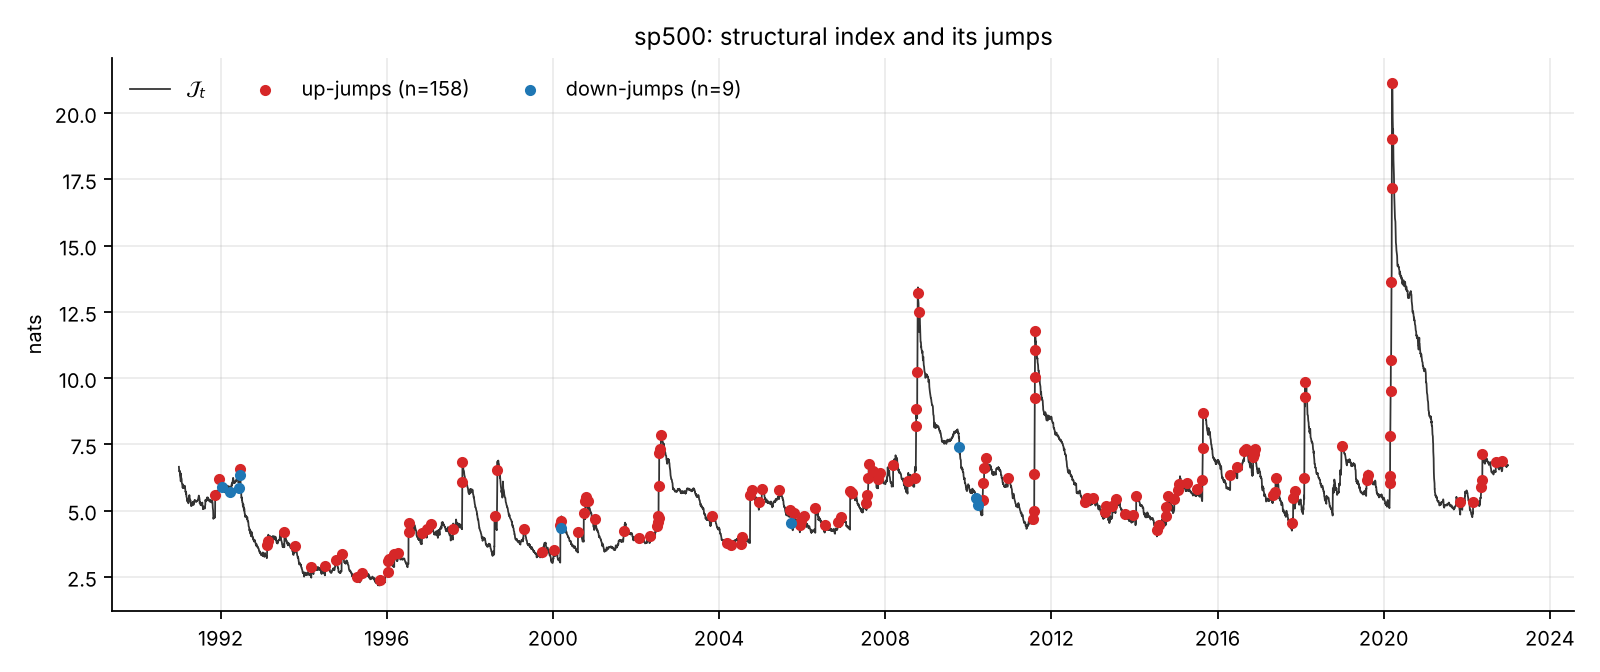
\includegraphics[width=0.6\linewidth]{figures/sp500_structural_index_jumps.png}
\caption{The structural index $\JJ_t$ on twenty S\&P~500 stocks, 1990--2022,
with detected jumps (red: rises, blue: falls). The sawtooth is visible, but
the i.i.d.\ null reproduces it.}
\label{fig:index}
\end{figure}


\section{Severity ladder, composition and reverse stress testing}
\label{oa:ladder}
\subsubsection{Calibrating the radius on the market itself}

It remains to choose $\eta$. We read it from the market's information flow,
that is, from how much the market itself revises its distribution over
21~days, $I^{(21)}_t=\KL{p_t}{p_{t-21}}$, measured on the same quantity as the
constraint (the portfolio distribution). Historical quantiles of this flow give
a radius for each return period (table~\ref{tab:ladder}).

\begin{table}[htbp]
\centering
\small
\begin{tabular}{@{}lrrrrrr@{}}
\toprule
Return period & 1~yr & 2~yrs & 5~yrs & 10~yrs & 20~yrs & 50~yrs$^\dagger$ \\
\midrule
radius $\eta$ (nats) & 0.017 & 0.045 & 0.149 & 0.408 & 0.634 & 1.369 \\
directional shock (std.\ dev.) & $-0.08$ & $-0.13$ & $-0.24$ & $-0.38$ & $-0.47$ & $-0.66$ \\
volatility multiplier & 1.12 & 1.20 & 1.37 & 1.63 & 1.80 & 2.21 \\
one-day ES$_{99}$ & $3.9\%$ & $4.2\%$ & $4.9\%$ & $5.9\%$ & $6.6\%$ & $8.3\%$ \\
\midrule
\emph{historical:} realised volatility increase & 1.54 & 1.77 & 2.28 & 3.25 & 3.57 & 4.43 \\
\bottomrule
\end{tabular}
\caption{Severity ladder for an equally weighted portfolio of the twenty
stocks, calibrated on the 21-day information flow (383 non-overlapping
observations). Current state: annual volatility $20\,\%$, one-day ES$_{99}$
$3.4\,\%$. Last row: quantile, at the same return period, of the ratio of
next-21-day volatility to past-252-day volatility. $^\dagger$ Extrapolated
beyond 33~years of data.}
\label{tab:ladder}
\end{table}

The scenario spends its budget mostly on volatility rather than direction: at
the ten-year rung, $63\,\%$ more volatility and a $0.38$-standard-deviation
shift, because ES is more sensitive to scale than to location. The radius
depends on the portfolio: a ladder must be calibrated for the portfolio it is
applied to.

\paragraph{A serious limit.} The last row confronts the ladder with history.
A ten-year scenario multiplies volatility by $1.6$, whereas the ten-year
quantile of the realised volatility increase is $3.2$. The ladder is therefore
\emph{too mild} by a factor close to two. Either the information flow,
measured on smoothed estimators, understates the true revision, or a Gaussian
ball is the wrong geometry for such abrupt volatility shocks. We do not
settle between the two. The return periods in the table must therefore not be
quoted as frequencies. What withstands this limit are the \emph{relative}
comparisons of the next two subsections.

\subsubsection{Composing a scenario: volatility or correlation?}
\label{sec:composition}

The entropy ball fixes the severity \emph{of the portfolio} (its stressed mean
and volatility). It does not say how each asset's covariance should move to
get there. The default choice, used so far, is a uniform dilation of
volatilities with correlations unchanged. That is a convention, not a fact
about crises. Yet section~5 of the main text shows that, under stress,
dependence moves on its own.

A simple property allows for this without changing severity. Portfolio
variance, $w^\top\Sigma w$, is linear in $\Sigma$. If two covariances give the
same portfolio variance, so does any mixture of the two (proposition in
Appendix~A of the main text). One can therefore mix an ``all-volatility''
covariance and an ``all-correlation'' covariance with a weight $\alpha$, the
\emph{dependence share}, without touching severity. One caveat: correlation
alone cannot carry any severity. With all correlations equal to one, our
portfolio's volatility cannot exceed $1.5$~times its current level; beyond
that, the rest comes from dilation.

The dependence share is calibrated on the robust results. The \emph{anchor}
comes from H1: under stress, dependence accounts for $0.99/(0.99+5.97)=14\,\%$
of the move in Gaussian entropy (scale plus dependence). The
\emph{refinement} comes from H8: over the more severe half of episodes, this
share reaches $49\,\%$.

\begin{table}[htbp]
\centering
\small
\begin{tabular}{@{}lrr@{}}
\toprule
Composition of the ten-year scenario ($\eta=0.41$) & dependence share & total cost (nats) \\
\midrule
default: uniform dilation & $0.00$ & $6.80$ \\
calibrated on H1 (regime average) & $0.14$ & $2.88$ \\
refined by H8 (severe episodes) & $0.49$ & $0.71$ \\
\bottomrule
\end{tabular}
\caption{Total cost in nats, on the twenty assets, of three compositions that
produce exactly the same portfolio severity (ES$_{99}=5.9\,\%$). On the French
industries: $14.7$, $8.3$ and $5.8$~nats for shares of $0$, $0.20$ and
$0.75$.}
\label{tab:composition}
\end{table}

The result is counter-intuitive (table~\ref{tab:composition}): the larger the
dependence share, the \emph{less} improbable the scenario, for the same
severity. Uniform dilation is therefore not a prudent choice; it is both less
realistic and more costly in plausibility than a composition anchored on
history. This finding is specific to this panel and should not be read as a
general law.

\subsubsection{Reverse stress testing}

The same unit also answers the reverse question: what is the least improbable
scenario that produces a given loss? On the main panel, the daily loss
exceeded one day in a hundred ($3.2\,\%$) costs $1.5$~nats; the one exceeded
one day in a thousand ($7.7\,\%$) costs $4.8$~nats; the worst day in 33~years
($11.5\,\%$) costs $9.0$~nats. Beyond a few nats, the non-parametric version
of this calculation rests on a handful of days, and the Gaussian version
should be preferred.


\section{Computing the cost in nats of the EBA 2025 adverse scenario}
\label{oa:eba}

Code: scripts/eba\_nats.py; results: paper/tables/eba\_nats.csv.

\paragraph{1. The shocks.} We take the adverse macro-financial scenario
\citep{eba2025} for 2025, as deviations from the baseline (annual averages):
EU equities $-50\,\%$, the baseline assuming them unchanged (table~4.1.7 of
the document); German long rate $3.50\,\%$ against $2.40\,\%$ and EU long
rate $4.80\,\%$ against $3.12\,\%$ (table~4.1.6); euro exchange rates against
the dollar, pound, yen and Swiss franc unchanged (table~4.1.10). Each shock is
mapped to the corresponding series of the euro-area panel
(section~\ref{oa:ciss}), giving an eleven-component vector $\Delta$:
\begin{center}
\small
\resizebox{\textwidth}{!}{\begin{tabular}{@{}llrrr@{}}
\toprule
EBA shock & Panel series & $\Delta_i$ & $\sigma_i$ (1 yr) & cost alone (nats) \\
\midrule
EU equities $-50\,\%$ & DAX, CAC~40, FTSE~MIB, IBEX~35, AEX & $\ln0.5=-0.693$ & $19$--$23\,\%$ & $4.4$--$6.5$ \\
German long rate & 10-year AAA yield (ECB) & $+1.10$~pt & $0.65$~pt & $1.4$ \\
EU long rate & 10-year all-ratings yield (ECB) & $+1.68$~pt & $0.68$~pt & $3.0$ \\
FX unchanged & EUR/USD, GBP, JPY, CHF & $0$ & $7$--$11\,\%$ & $0$ \\
\bottomrule
\end{tabular}}
\end{center}
Equities as log returns, rates as level changes; the maturity of long rates is
not specified by the document and is taken at ten years. GDP, unemployment,
real estate and inflation, which are not market prices, are not used.

\paragraph{2. The reference.} $p_0=\mathcal N(0,\Sigma)$, where $\Sigma$ is
the covariance of one-year changes in the eleven series, estimated on daily
changes from 6~September 2004 to 31~December 2024 (the data available to the
designer) and multiplied by 252.

\paragraph{3. The formula.} The scenario fixes means, not volatilities or
correlations. We read it as a pure mean shift, hence
(Appendix~A of the main text) $\KL{p_{\text{scenario}}}{p_0}=\tfrac12\Delta^\top
\Sigma^{-1}\Delta$. This is the \emph{minimal} cost consistent with the
scenario: among all distributions with mean $\Delta$, the shifted Gaussian is
the closest to $p_0$. Unspecified variables (two- and five-year rates, banks,
etc.) are left free; filling them with their conditional expectation is the
cheapest choice, and the cost then depends only on the shocked block $S$:
$\tfrac12\Delta_S^\top\Sigma_{SS}^{-1}\Delta_S$. The cost of a single variable
is $\tfrac12(\Delta_i/\sigma_i)^2$; for the DAX ($\sigma=20.3\,\%$), the shock
is $3.4$~standard deviations and costs $5.8$~nats. Read $\eta$~nats as
$\sqrt{2\eta}$~standard deviations.

\begin{table}[t]
\centering
\small
\begin{tabular}{@{}lrr@{}}
\toprule
Cost in nats & equities and rates & with FX fixed \\
\midrule
\textbf{EBA 2025 adverse scenario, year 1} & $\mathbf{10.5}$ & $\mathbf{11.1}$ \\
\quad equities only / rates only & $6.8$ / $3.1$ & \\
\quad sum of variable-by-variable costs & $31.9$ & \\
\midrule
\emph{Observed years:} 2011 / 2008 / 2022 & $3.1$ / $11.2$ / $11.9$ & $3.1$ / $18.2$ / $13.2$ \\
\quad worst rolling year (March 2008--March 2009) & $14.4$ & $19.5$ \\
\bottomrule
\end{tabular}
\caption{Cost in nats of the EBA 2025 adverse scenario and of observed years,
on five equity indices, two ten-year rates and four exchange rates, with the
annual covariance estimated on 2004--2024.}
\label{tab:eba}
\end{table}

\paragraph{4. Reading.} The sum of variable-by-variable costs is
$31.9$~nats, the joint cost $10.5$: a common shock to highly correlated indices
follows the most likely direction in the data. Equities alone ($6.8$) plus
rates alone ($3.1$) leave $0.5$~nat of interaction (falling equities with
rising rates go against the historical correlation, $+0.13$). Fixing FX adds
$0.7$~nat.

\paragraph{5. Observed years.} Same calculation, same $\Sigma$, on the
realised changes of the eleven series (31~December to 31~December; worst
252-day window ending 17~March 2009). The median year costs $4.1$~nats. The
scenario combines the equity fall of 2008 (when rates fell) and the rate rise
of 2022 (close to $3$~points).

\paragraph{6. Variants} (equities and rates / with FX fixed). Covariance of
rolling annual changes: $12.8$ / $18.7$; sample to 2026: $10.6$ / $11.3$;
crisis covariance 2008--2012: $8.4$ / $9.0$. At the end of the three-year
horizon (2027: $-42\,\%$, $+87$ and $+112$~bp, three-year covariance), the cost
falls to $2.1$ / $2.2$: severity is concentrated in the first year.

\paragraph{7. Limits.} Shocks in annual averages; the EU equity fall applied
to each index; a Gaussian reference without fat tails, which tends to
overstate the cost. The ECB's instantaneous market-risk scenario is not priced
(detailed tables not accessible), but the same formula applies. These costs
(eleven series, one year) are not directly comparable with
table~\ref{tab:ladder} (equity portfolio, 21~days).


\section{The entropic CISS: a euro-area application of the block decomposition}
\label{oa:ciss}

The paper's one robust result, coupling under stress, becomes here an
indicator in the format of the ECB's CISS \citep{hollo2012}. Like the CISS, it
covers the money market, bond, equity, financial intermediary and foreign
exchange segments. Unlike the CISS, it says which share of coupling lies
within each segment and which lies \emph{between} segments. For a scenario
designer, this is precisely the information needed to set correlations
between shocks to different markets.

\subsection{An exact decomposition by segment}

Split the series into segments $B_1,\dots,B_K$. Total coupling decomposes
exactly:
\begin{equation}
\label{eq:blocks}
C(R) \;=\; \underbrace{\sum_{k=1}^{K} C(R_{kk})}_{\text{within segments}}
\;+\; \underbrace{I(B_1;\dots;B_K)}_{\text{between segments}},
\end{equation}
where $R_{kk}$ is the correlation matrix of segment $k$. The between-segment
term is zero exactly when the segments move independently of one another: it
is the systemic part. For two segments $A$ and $B$, the mutual information
$I(A;B)$ gives a contagion map in the same unit. Everything is unit-free:
equity returns, rate changes and exchange rates can sit in the same matrix. We
use the rank version of coupling.

\subsection{The euro-area panel}

The panel is daily, from January 2005 to October 2026 (5,690 days), with
28~series: the overnight rate (EONIA, then \texteuro{}STR) for the money
market; six ECB sovereign yields and spreads for bonds; five national indices
for equities; nine banks and three insurers for intermediaries; four euro
exchange rates. The CISS uses the Euribor minus overnight spread for the money
market; since Euribor is not available on the ECB portal, this segment for now
contains only the overnight rate.

\subsection{Results}

\begin{table}[htbp]
\centering\small
\resizebox{\linewidth}{!}{%
\begin{tabular}{@{}lrrrrr@{}}\toprule
& Rise under & \multicolumn{2}{c}{i.i.d.\ null} & \multicolumn{2}{c}{CCC-FHS null} \\
\cmidrule(lr){3-4}\cmidrule(lr){5-6}
Component & stress (nats) & mean & $p$ & mean & $p$ \\\midrule
Total coupling & +1.61 & +0.20 & <0.001 & +0.32 & <0.001 \\
\textbf{Between segments} & +0.19 & +0.02 & <0.001 & +0.03 & 0.002 \\
Within: equities & +0.46 & +0.05 & <0.001 & +0.08 & <0.001 \\
Within: intermediaries & +0.48 & +0.13 & <0.001 & +0.21 & 0.020 \\
Within: bonds & +0.34 & -0.01 & <0.001 & +0.00 & <0.001 \\
Within: FX & +0.14 & +0.00 & <0.001 & +0.00 & <0.001 \\
Equities -- intermediaries & +0.096 & +0.010 & <0.001 & +0.016 & 0.012 \\
Bonds -- FX & +0.055 & +0.004 & <0.001 & +0.005 & 0.002 \\
Bonds -- intermediaries & +0.040 & +0.003 & <0.001 & +0.008 & 0.016 \\
Bonds -- equities & +0.029 & +0.003 & 0.002 & +0.004 & 0.013 \\
Equities -- FX & +0.046 & +0.006 & <0.001 & +0.005 & 0.002 \\
Intermediaries -- FX & +0.040 & +0.007 & <0.001 & +0.006 & 0.004 \\
Money market -- other segments & $\approx 0$ & $\approx 0$ & n.s. & $\approx 0$ & n.s. \\
\bottomrule\end{tabular}}
\caption{Euro area: stress-minus-calm rise of each coupling component against the two placebo nulls
(999 replications each; $p$ exact, one-sided). Stress is the top decile of equity-block volatility, with
the threshold computed on the past only. The CCC-FHS null fits a GJR-GARCH(1,1) to each of the 28 series.}
\label{tab:cb-euro}
\end{table}


\begin{figure}[htbp]
\centering
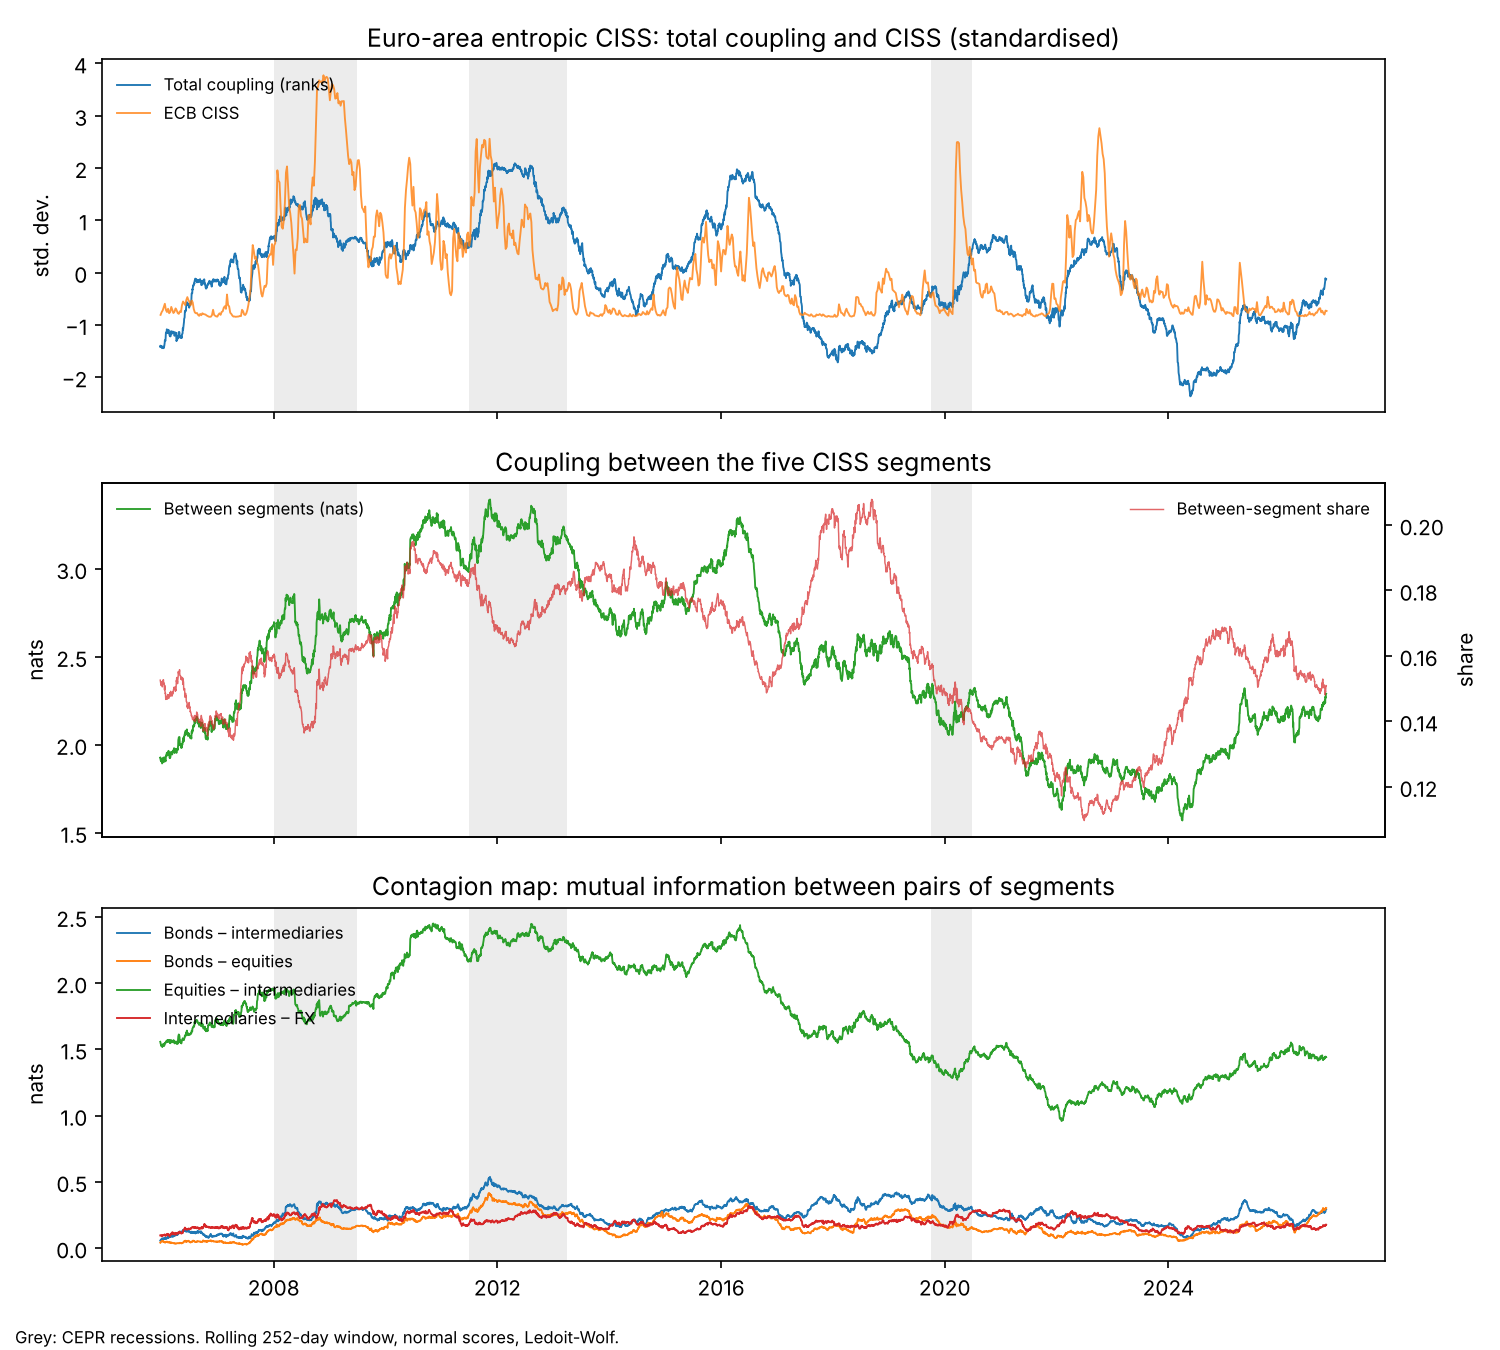
\includegraphics[width=0.8\linewidth]{figures/euro_ciss_entropique_overnight_only_en.png}
\caption{The euro-area entropic CISS. Top: total coupling and the ECB's CISS,
standardised. Middle: coupling between the five segments, in nats, and its
share of the total. Bottom: mutual information between pairs of segments.
Grey areas: CEPR recessions.}
\label{fig:cb-euro}
\end{figure}

Three readings (table~\ref{tab:cb-euro} and figure~\ref{fig:cb-euro}).
\begin{itemize}
\item \emph{Stress ties segments together}, far beyond both nulls: the
between-segment rise is nine times the i.i.d.\ null's and six times that of
the volatility-preserving null, which keeps each series' GARCH dynamics. Every
pair outside the money market rises beyond both nulls; the links between
equities and intermediaries and with FX are the clearest. The weakest result
is coupling within the intermediaries block ($p=\euIntermFhsP$ against the
volatility-preserving null): bank and insurer stocks move together partly
because their volatilities rise together.
\item \emph{The sovereign--bank link stands out.} Mutual information between
bonds and intermediaries peaks in late 2011, at the height of the sovereign
debt crisis ($0.46$~nat against $0.10$ in late 2006). The aggregate CISS
cannot show which segments an episode ties together.
\item \emph{The money market does not couple} in daily data: the overnight
rate follows monetary policy, not market stress.
\end{itemize}

\begin{table}[htbp]
\centering
\small
\resizebox{\linewidth}{!}{%
\begin{tabular}{@{}lcccc@{}}
\toprule
& Total coupling & Between segments & Volatility & CISS \\
\midrule
Correlation with the CISS & $0.58$ & $0.35$ & $0.74$ & $1$ \\
AUROC, CEPR recessions & $\mathbf{0.85}$ & $0.75$ & $0.80$ & $0.83$ \\
Explains the CISS beyond volatility ($t$) & $\mathbf{6.7}$ & $1.7$ & & \\
Growth-at-Risk, alone: $p$ & $0.04$ & $<0.001$ & $0.98$ & $<0.001$ \\
Growth-at-Risk, with CISS and past growth: $p$ & $0.78$ & $0.81$ & & $<0.001$ \\
\bottomrule
\end{tabular}}
\caption{Euro area against official indicators. The AUROC is the probability
that a randomly drawn recession date has a higher indicator than a
non-recession date ($0.5$: no power; $1$: perfect separation).
Growth-at-Risk: regression of the bottom decile of four-quarter GDP growth on
the indicator \citep{adrian2019}, 79~quarters.}
\label{tab:cb-official}
\end{table}

Against official indicators (table~\ref{tab:cb-official}), total coupling
flags recessions slightly better than the CISS and volatility, and it explains
the CISS beyond what volatility explains. It does not, however, forecast
growth once the CISS is accounted for. With three recessions and
79~quarters, these comparisons are indicative. The indicator is therefore
\emph{coincident}: a complement to the CISS that says which segments are
linked, not a better predictor. On US data, against the St.~Louis Fed stress
index \citep{kliesen2010}, coupling adds to volatility on the twenty stocks
($t\approx4$ to $5$), mainly before 2015, but not on the 48~industries.

\paragraph{Next steps.} Add Euribor from its administrator (EMMI) to rebuild
the money-market segment as in the CISS; date stress episodes with the ESRB
crisis database \citep{loduca2017} and measure how the contagion map behaves
around them; compare the indicator with institution-level systemic-risk
measures, SRISK \citep{brownlees2017} and $\Delta$CoVaR \citep{adrian2016}.


\bibliographystyle{chicago}
\bibliography{references}
\end{document}
